\documentclass[12pt, a4paper]{article}

% ── Packages ──────────────────────────────────────────────────────
\usepackage{fontspec}
\setmainfont{Arial}
\usepackage{amsmath, amssymb, amsthm}
\usepackage{mathtools}
\usepackage{enumitem}
\usepackage{tikz}
\usetikzlibrary{calc, positioning, arrows.meta, fit, patterns, decorations.pathreplacing}
\usepackage{geometry}
\geometry{margin=2.4cm}
\usepackage{xcolor}
\usepackage{tcolorbox}
\tcbuselibrary{theorems, skins, breakable}
\usepackage{booktabs}
\usepackage{hyperref}
\hypersetup{colorlinks=true, linkcolor=blue!60!black, urlcolor=blue!60!black}

\setlength{\parindent}{0pt}
\setlength{\parskip}{6pt}

% ── Colours ───────────────────────────────────────────────────────
\definecolor{setA}{RGB}{66, 133, 244}   % blue
\definecolor{setB}{RGB}{234, 67, 53}    % red
\definecolor{setC}{RGB}{251, 188, 4}    % yellow
\definecolor{theoryBg}{RGB}{232, 245, 253}
\definecolor{theoryFrame}{RGB}{66, 133, 244}
\definecolor{stmtBg}{RGB}{255, 243, 224}
\definecolor{stmtFrame}{RGB}{230, 126, 34}
\definecolor{ansBg}{RGB}{232, 250, 232}
\definecolor{ansFrame}{RGB}{39, 174, 96}

% ── Environments ──────────────────────────────────────────────────
\newtcolorbox{theorybox}[1][]{%
  colback=theoryBg, colframe=theoryFrame,
  fonttitle=\bfseries, title={\small Տեսության ամփոփում. #1},
  breakable, enhanced, arc=2mm,
  left=5pt, right=5pt, top=5pt, bottom=5pt
}

\newtcolorbox{problembox}{%
  colback=stmtBg, colframe=stmtFrame,
  fonttitle=\bfseries, title={\small Խնդրի դրվածք},
  breakable, enhanced, arc=2mm,
  left=5pt, right=5pt, top=5pt, bottom=5pt
}

\newtcolorbox{answerbox}{%
  colback=ansBg, colframe=ansFrame,
  arc=2mm, left=5pt, right=5pt, top=3pt, bottom=3pt
}

\newcommand{\Z}{\mathbb{Z}}
\newcommand{\R}{\mathbb{R}}
\newcommand{\N}{\mathbb{N}}
\newcommand{\powset}[1]{2^{#1}}
\newcommand{\comp}[1]{\overline{#1}}
\newcommand{\symdiff}{\mathbin{\triangle}}

% ── Title ─────────────────────────────────────────────────────────
\title{\textbf{Գործնական 1 — Բազմությունների տեսություն}\\[4pt]
       \large Ընտրված խնդիրների լուծումներ\\[2pt]
       \normalsize Խնդիրներ 2, 7, 11, 16, 20, 54\,(3,\,11), 58, 60}
\author{Դիսկրետ մաթեմատիկա — ԵՊՀ}
\date{}

\begin{document}
\maketitle
\tableofcontents
\newpage

% ══════════════════════════════════════════════════════════════════
\section{Խնդիր 2 — Պատկանելիություն $\varnothing$-ի և $\{\varnothing\}$-ի հետ}
% ══════════════════════════════════════════════════════════════════

\begin{theorybox}[Պատկանելիություն ($\in$) թե՞ ենթաբազմություն ($\subseteq$)]
Այս երկու հարաբերությունները սկզբունքորեն տարբեր են։
\begin{itemize}[nosep]
  \item $a \in S$ նշանակում է «$a$-ն $S$-ի \textbf{տարր} է»։
  \item $A \subseteq S$ նշանակում է «$A$-ի յուրաքանչյուր տարր նաև $S$-ի մեջ է»։
\end{itemize}

\medskip
Դատարկ բազմությունը՝ $\varnothing$, տարրեր չունի։
$\{\varnothing\}$ բազմությունը դատարկ \textbf{չէ}։ այն ունի մեկ տարր, որն էլ հենց $\varnothing$-ն է։
Անմիջականորեն պարզելու համար՝ արդյոք $x \in S$, թվարկեք $S$-ի տարրերը և տեսեք՝ արդյոք $x$-ը դրանց թվում է։

\begin{center}
\begin{tikzpicture}[
  box/.style={draw, rounded corners=3pt, minimum width=2.4cm,
              minimum height=1.1cm, align=center, font=\small},
  >=Stealth
]
  \node[box, fill=gray!8] (e0)
    {$\varnothing = \{\,\}$\\[-1pt]\footnotesize 0 տարր};
  \node[box, fill=setA!8, right=1.6cm of e0] (e1)
    {$\{\varnothing\}$\\[-1pt]\footnotesize 1 տարր՝ $\varnothing$};
  \node[box, fill=setB!8, right=1.6cm of e1] (e2)
    {$\{\{\varnothing\}\}$\\[-1pt]\footnotesize 1 տարր՝ $\{\varnothing\}$};
  \draw[->, thick, gray!70!black] (e0) -- (e1)
    node[midway, above, font=\footnotesize]{ներառել փակագծերում};
  \draw[->, thick, gray!70!black] (e1) -- (e2)
    node[midway, above, font=\footnotesize]{ներառել փակագծերում};
\end{tikzpicture}
\end{center}
Յուրաքանչյուր փաթեթավորման քայլ ստեղծում է նոր բազմություն, որի միակ տարրը նախորդ բազմությունն է։
\end{theorybox}

\begin{problembox}
Հետևյալ պնդումներից որո՞նք են ճիշտ։
\begin{enumerate}[label=2.\arabic*.]
  \item $\varnothing \in \{\varnothing,\; \{\varnothing\}\}$
  \item $\{\varnothing\} \in \{\{\varnothing\}\}$
  \item $\varnothing \in \{\{\varnothing\}\}$
\end{enumerate}
\end{problembox}

\medskip
\begin{tcolorbox}[colback=blue!3, colframe=setA!60!black, arc=2mm, left=5pt, right=5pt, top=5pt, bottom=5pt, title={\small Արկղի անալոգիա. Ինչպե՞ս է աշխատում $\in$-ը}]
Պատկերացրեք յուրաքանչյուր բազմություն որպես \textbf{արկղ}։ $\in$ օպերատորը բացում է արկղը և նայում, թե ինչ կա \emph{անմիջապես} ներսում։ այն նայում է միայն \textbf{մեկ մակարդակ խորությամբ}։ Այն երբեք չի բացում ներսի արկղերը։

\begin{itemize}[nosep]
  \item $\varnothing$-ն \textbf{դատարկ արկղ} է։ բացում եք և ներսում ոչինչ չեք գտնում։
        Հետևաբար $|\varnothing| = 0$։
  \item $\{\varnothing\}$-ն \textbf{մեկ իր պարունակող արկղ} է՝ մեկ այլ (դատարկ) արկղ։
        Բացում եք $\{\varnothing\}$-ն և տեսնում եք մեկ բան՝ դատարկ $\varnothing$ արկղը։
        Հետևաբար $|\{\varnothing\}| = 1$։
\end{itemize}

\medskip
Ահա թե ինչու $\varnothing \neq \{\varnothing\}$. դատարկ արկղը նույնը չէ, ինչ դատարկ արկղ պարունակող արկղը, ճիշտ այնպես, ինչպես դատարկ ծրարը նույնը չէ, ինչ մեկ այլ դատարկ ծրար պարունակող ծրարը։

Երբ ստուգում եք «$x \in S$», բացեք $S$ արկղը, նայեք անմիջապես տեսանելի իրերին (մեկ մակարդակ խորությամբ) և ստուգեք, թե արդյոք $x$-ը դրանցից մեկն է։ \textbf{Երբեք մի բացեք իրերի ներսում գտնվող իրերը։}
\end{tcolorbox}

\medskip
\textbf{Մեթոդ.} Նախ թվարկեք յուրաքանչյուր արտաքին բազմության տարրերը՝ $\{\varnothing,\;\{\varnothing\}\}$, $\{\{\varnothing\}\}$: Այնուհետև ստուգեք, թե արդյոք $\in$-ի ձախ կողմի օբյեկտը համընկնում է թվարկված որևէ տարրի հետ։

\subsection*{Լուծում}

Ռազմավարությունը միշտ նույնն է։ \emph{թվարկեք արտաքին բազմության տարրերը},
ապա ստուգեք, թե արդյոք $\in$-ի ձախ կողմի օբյեկտը համընկնում է դրանցից որևէ մեկի հետ։

\begin{center}
\begin{tikzpicture}[
  elem/.style={draw, rounded corners=4pt, minimum width=1.1cm,
               minimum height=0.9cm, inner sep=2pt, font=\small, align=center},
  container/.style={draw, rounded corners=8pt, inner sep=12pt, thick},
  >=Stealth
]
  % ── 2.1 ──
  \begin{scope}[xshift=0cm]
    \node[font=\footnotesize\bfseries] at (0.55, 2.6) {2.1};
    \node[elem, fill=setA!15] (a1) at (0, 0.7) {$\varnothing$};
    \node[elem, fill=setB!15] (a2) at (1.1, 0.7) {$\{\varnothing\}$};
    \node[container, fit=(a1)(a2),
          label={[font=\scriptsize, yshift=4pt]above:$\{\varnothing,\;\{\varnothing\}\}$}] {};
    \draw[->, thick, setA!70!black]
      (0, -0.7) node[below, font=\scriptsize]{$\varnothing$} -- (a1.south);
    \node[font=\scriptsize\bfseries, green!50!black] at (0.55, -1.5)
      {Համընկնում է $\checkmark$ \;\textbf{ՃԻՇՏ Է}};
  \end{scope}

  % ── 2.2 ──
  \begin{scope}[xshift=4.3cm]
    \node[font=\footnotesize\bfseries] at (0, 2.6) {2.2};
    \node[elem, fill=setB!15] (b1) at (0, 0.7) {$\{\varnothing\}$};
    \node[container, fit=(b1),
          label={[font=\scriptsize, yshift=4pt]above:$\{\{\varnothing\}\}$}] {};
    \draw[->, thick, setB!70!black]
      (0, -0.7) node[below, font=\scriptsize]{$\{\varnothing\}$} -- (b1.south);
    \node[font=\scriptsize\bfseries, green!50!black] at (0, -1.5)
      {Համընկնում է $\checkmark$ \;\textbf{ՃԻՇՏ Է}};
  \end{scope}

  % ── 2.3 ──
  \begin{scope}[xshift=8cm]
    \node[font=\footnotesize\bfseries] at (0, 2.6) {2.3};
    \node[elem, fill=setB!15] (c1) at (0, 0.7) {$\{\varnothing\}$};
    \node[container, fit=(c1),
          label={[font=\scriptsize, yshift=4pt]above:$\{\{\varnothing\}\}$}] {};
    \draw[->, thick, red!70!black]
      (0, -0.7) node[below, font=\scriptsize]{$\varnothing$} -- (c1.south);
    \node[font=\scriptsize\bfseries, red!70!black] at (0, -1.5)
      {$\varnothing \neq \{\varnothing\}$ \;\textbf{ՍԽԱԼ Է}};
  \end{scope}
\end{tikzpicture}
\end{center}

\begin{center}
\renewcommand{\arraystretch}{1.4}
\begin{tabular}{lll}
\toprule
\textbf{Ձախ օբյեկտ} & \textbf{Արտաքին բազմության տարրեր} & \textbf{Համընկնո՞ւմ են} \\
\midrule
$\varnothing$ & $\varnothing,\;\{\varnothing\}$ & Այո — \textbf{ՃԻՇՏ Է} \\
$\{\varnothing\}$ & $\{\varnothing\}$ & Այո — \textbf{ՃԻՇՏ Է} \\
$\varnothing$ & $\{\varnothing\}$ & Ոչ ($\varnothing \neq \{\varnothing\}$) — \textbf{ՍԽԱԼ Է} \\
\bottomrule
\end{tabular}
\end{center}

\textbf{2.1.}\; $\varnothing \in \{\varnothing,\;\{\varnothing\}\}$
\;---\; \textbf{ՃԻՇՏ Է։}
Բազմությունն ունի երկու տարր՝ $\varnothing$ և $\{\varnothing\}$։
$\varnothing$ օբյեկտը հստակորեն դրանցից մեկն է։

\textbf{2.2.}\; $\{\varnothing\} \in \{\{\varnothing\}\}$
\;---\; \textbf{ՃԻՇՏ Է։}
$\{\{\varnothing\}\}$ բազմությունն ունի ճիշտ մեկ տարր՝ $\{\varnothing\}$։
Ձախ կողմի օբյեկտը $\{\varnothing\}$-ն է, որը համընկնում է։

\textbf{2.3.}\; $\varnothing \in \{\{\varnothing\}\}$
\;---\; \textbf{ՍԽԱԼ Է։}
Միակ տարրը $\{\varnothing\}$-ն է։
Մեզ պետք է, որ $\varnothing = \{\varnothing\}$, բայց $|\varnothing|=0$, մինչդեռ $|\{\varnothing\}|=1$,
ուստի դրանք հավասար չեն։

\begin{answerbox}
\centering 2.1 — Ճիշտ է \qquad 2.2 — Ճիշտ է \qquad 2.3 — Սխալ է
\end{answerbox}

% ══════════════════════════════════════════════════════════════════
\section{Խնդիր 7 — $\in$-ը տրանզիտիվ չէ}
% ══════════════════════════════════════════════════════════════════

\begin{theorybox}[$\in$-ը տրանզիտիվ չէ]
$\subseteq$-ը \textbf{տրանզիտիվ է}.
$A \subseteq B \land B \subseteq C \;\Longrightarrow\; A \subseteq C$.

$\in$-ը \textbf{տրանզիտիվ չէ}.
$A \in B \land B \in C \;\not\Longrightarrow\; A \in C$.

\medskip
\textbf{Ինչո՞ւ:} $\in$-ը հատում է ներդրման մեկ «մակարդակ»։
Երկու հաջորդական $\in$ քայլերը հատում են երկու մակարդակ, ուստի $A$-ն ներդրված է $C$-ի մեջ,
սակայն վերջինիս անմիջական տարրը չէ։

\begin{center}
\begin{tikzpicture}[font=\small, >=Stealth]
  % Three nested boxes with clear level labels
  \fill[setC!8, rounded corners=10pt] (-0.2,-0.2) rectangle (8.2, 3.4);
  \draw[thick, setC!70!black, rounded corners=10pt] (-0.2,-0.2) rectangle (8.2, 3.4);
  \node[anchor=north west, font=\footnotesize\bfseries, setC!70!black] at (0, 3.3) {$C$};

  \fill[setB!10, rounded corners=7pt] (0.3, 0.3) rectangle (5.7, 2.7);
  \draw[thick, setB!70!black, rounded corners=7pt] (0.3, 0.3) rectangle (5.7, 2.7);
  \node[anchor=north west, font=\footnotesize\bfseries, setB!70!black] at (0.5, 2.6) {$B$};

  \fill[setA!15, rounded corners=4pt] (0.8, 0.7) rectangle (2.6, 2.1);
  \draw[thick, setA!70!black, rounded corners=4pt] (0.8, 0.7) rectangle (2.6, 2.1);
  \node[font=\bfseries, setA!70!black] at (1.7, 1.4) {$A$};

  % Other elements
  \node[font=\small, gray] at (4.2, 1.4) {$2$};
  \node[font=\small, gray] at (7.0, 1.6) {$3$};

  % Annotations
  \draw[<-, thick, setA!70!black] (1.7, 0.55) -- (1.7, -0.6)
    node[below, font=\footnotesize]{$A \in B$ (մակարդակ 1)};
  \draw[<-, thick, setB!70!black] (3.8, 0.15) -- (3.8, -1.1)
    node[below, font=\footnotesize]{$B \in C$ (մակարդակ 2)};
  \node[font=\footnotesize, red!70!black, align=center] at (7.0, -1.1)
    {$A$-ն $C$-ի անմիջական\\տարր \emph{չէ}};
\end{tikzpicture}
\end{center}
\end{theorybox}

\begin{problembox}
Բերեք $A$, $B$, $C$ բազմությունների օրինակներ, որտեղ
$A \in B$, \;$B \in C$, \;բայց $A \notin C$.
\end{problembox}

\begin{tcolorbox}[colback=yellow!5, colframe=stmtFrame!80!black, arc=2mm, left=5pt, right=5pt, top=5pt, bottom=5pt, title={\small Իրական աշխարհի անալոգիա. Մակարդակների թռիչքներ}]
\textbf{Անձ, հանձնաժողով և աշխատանքային խումբ:}

Ենթադրենք Պրոֆեսոր $A$-ն Ուսումնական հանձնաժողով $B$-ի \emph{անդամ} է, իսկ Ուսումնական հանձնաժողով $B$-ն Համալսարանի աշխատանքային խումբ $C$-ի \emph{անդամ} է (մարմին, որի անդամները ամբողջական հանձնաժողովներ են, այլ ոչ թե անհատ մարդիկ):

\begin{itemize}[nosep]
  \item $A \in B$: պրոֆեսորը հանձնաժողովի կազմում է։
  \item $B \in C$: հանձնաժողովը աշխատանքային խմբի կազմում է։
  \item $A \notin C$: պրոֆեսորը անհատապես աշխատանքային խմբի անդամ \textbf{չէ}։ միայն ամբողջական հանձնաժողովներն են աշխատանքային խմբի անդամ։
\end{itemize}

Հիմնական գաղափարը. $\in$-ը հատում է պարունակության ճիշտ \textbf{մեկ մակարդակ}։ Երկու $\in$-քայլերը հատում են \emph{երկու} մակարդակ, ուստի անհատը ($A$) թաղված է $C$-ի ներսում երկու մակարդակ խորությամբ, բայց $C$-ի \emph{ուղղակի} անդամ չէ։
\end{tcolorbox}

\subsection*{Լուծում}
Դիցուք՝
\[
  A = 1, \qquad B = \{1, 2\}, \qquad C = \bigl\{\{1, 2\},\; 3\bigr\}.
\]

\begin{center}
\renewcommand{\arraystretch}{1.4}
\begin{tabular}{lll}
\toprule
\textbf{Պայման} & \textbf{Ստուգում} & \textbf{Արդյունք} \\
\midrule
$A \in B$ & Արդյո՞ք $1 \in \{1, 2\}$: & Այո $\checkmark$ \\
$B \in C$ & Արդյո՞ք $\{1,2\} \in \bigl\{\{1,2\},\, 3\bigr\}$: & Այո $\checkmark$ \\
$A \notin C$ & Արդյո՞ք $1 \in \bigl\{\{1,2\},\, 3\bigr\}$:
  Տարրերն են՝ $\{1,2\}$ և $3$: & $1 \notin C$ \;$\checkmark$ \\
\bottomrule
\end{tabular}
\end{center}

\textbf{Հիմնական գաղափար.}\;
$1$ թիվը $B$-ի տարր է, իսկ $B$-ն՝ $C$-ի տարր,
բայց $C$-ի տարրերն են $\{1,2\}$-ը (բազմություն) և $3$-ը (թիվ)։
$1$ թիվը դրանցից ոչ մեկը չէ, ուստի $1 \notin C$։

\medskip
\textbf{Հակադրություն.}\; $A \notin C$ եզրակացությունը ավտոմատ չէ։ այն կարող է չիրականանալ։
Դիցուք՝ $A = 1$, $B = \{1\}$, $C = \{1, \{1\}\}$։
Այդ դեպքում $A \in B$ ($1 \in \{1\}$), $B \in C$ ($\{1\} \in \{1, \{1\}\}$),
և նաև $A \in C$ ($1 \in \{1, \{1\}\}$)։
Այսպիսով, $\in$-ը երբեմն \emph{պատահաբար} կարող է լինել տրանզիտիվ, բայց ոչ միշտ։

% ══════════════════════════════════════════════════════════════════
\section{Խնդիր 11 — $\in$-ի և $\subseteq$-ի խառնուրդ}
% ══════════════════════════════════════════════════════════════════

\begin{theorybox}[$\in$-ի և $\subseteq$-ի խառնուրդ]
Երկու հարաբերությունները գործում են տարբեր «մակարդակներում»։
\begin{itemize}[nosep]
  \item $A \subseteq B$: երկուսն էլ գտնվում են նույն մակարդակում։ $A$-ի յուրաքանչյուր տարր
        նաև $B$-ի տարր է։
  \item $B \in C$: $B$-ն ինքնին դառնում է օբյեկտ $C$-ի ներսում։ թռիչք մեկ մակարդակ \emph{վեր}։
\end{itemize}

\begin{center}
\begin{tikzpicture}[font=\small, >=Stealth, node distance=1.8cm]
  \node[draw, rounded corners, fill=setA!10, minimum width=1.2cm] (A) {$A$};
  \node[draw, rounded corners, fill=setA!10, minimum width=1.2cm, right=of A] (B) {$B$};
  \node[draw, rounded corners, fill=setB!10, minimum width=1.2cm, right=of B] (C) {$C$};
  \node[draw, rounded corners, fill=setB!10, minimum width=1.2cm, right=of C] (D) {$D$};
  \node[draw, rounded corners, fill=setB!10, minimum width=1.2cm, right=of D] (E) {$E$};

  \draw[->, thick, setA!70!black] (A) -- (B)
    node[midway, above, font=\footnotesize]{$\subseteq$}
    node[midway, below, font=\tiny, gray]{նույն մակարդակ};
  \draw[->, thick, red!60!black, dashed] (B) -- (C)
    node[midway, above, font=\footnotesize]{$\in$}
    node[midway, below, font=\tiny, gray]{մակարդակի թռիչք};
  \draw[->, thick, setC!80!black] (C) -- (D)
    node[midway, above, font=\footnotesize]{$\subseteq$};
  \draw[->, thick, setC!80!black] (D) -- (E)
    node[midway, above, font=\footnotesize]{$\subseteq$};
\end{tikzpicture}
\end{center}
\end{theorybox}

\begin{problembox}
Բերեք $A, B, C, D, E$ բազմությունների օրինակներ, որոնք բավարարում են.
\[
  A \subseteq B, \quad B \in C, \quad C \subseteq D, \quad D \subseteq E:
\]
\end{problembox}

\subsection*{Լուծում}

\begin{tcolorbox}[colback=gray!3, colframe=gray!60, arc=2mm, left=5pt, right=5pt, top=5pt, bottom=5pt, title={\small Գունային ուղեցույց. Ներդրված մակարդակների տեսանելիություն}]
Երբ բազմությունները պարունակում են այլ բազմություններ որպես տարրեր, օգտակար է մակարդակները գունավորել։
\begin{itemize}[nosep]
  \item \textcolor{blue}{Կապույտ} = սովորական թվեր (ամենացածր մակարդակի օբյեկտներ):
  \item \textcolor{red}{Կարմիր փակագծեր} = ներքին բազմության ձևավոր փակագծեր, որը ինքնին արտաքին բազմության \emph{տարր} է։
  \item Սև փակագծեր = արտաքին բազմության սահմանները։
\end{itemize}

\medskip
Օրինակ՝ $C = \bigl\{\textcolor{red}{\{}\textcolor{blue}{1,2}\textcolor{red}{\}},\;\textcolor{blue}{3}\bigr\}$ ունի երկու տարր։
$\textcolor{red}{\{}\textcolor{blue}{1,2}\textcolor{red}{\}}$ բազմությունը (ներքին բազմություն, նշված կարմիր փակագծերով) և $\textcolor{blue}{3}$ թիվը (սովորական թիվ կապույտով)։

\medskip
Նմանապես՝
\[
  D = \bigl\{\textcolor{red}{\{}\textcolor{blue}{1,2}\textcolor{red}{\}},\;\textcolor{blue}{3},\;\textcolor{blue}{4}\bigr\},
  \qquad
  E = \bigl\{\textcolor{red}{\{}\textcolor{blue}{1,2}\textcolor{red}{\}},\;\textcolor{blue}{3},\;\textcolor{blue}{4},\;\textcolor{blue}{5}\bigr\}
\]
Յուրաքանչյուր դեպքում \textcolor{red}{կարմիր փակագծերով} տարրը բազմության տեսքով տարր է (մեկ մակարդակ վեր), իսկ \textcolor{blue}{կապույտ} տարրերը թվեր են։
\end{tcolorbox}

\[
  A = \{1\}, \quad B = \{1,2\}, \quad C = \bigl\{\{1,2\},\;3\bigr\}, \quad
  D = \bigl\{\{1,2\},\;3,\;4\bigr\}, \quad E = \bigl\{\{1,2\},\;3,\;4,\;5\bigr\}
\]

\begin{center}
\renewcommand{\arraystretch}{1.35}
\begin{tabular}{lcp{7.5cm}}
\toprule
\textbf{Պայման} & \textbf{Տիպ} & \textbf{Ստուգում} \\
\midrule
$A \subseteq B$ & ենթաբազմություն &
  $\{1\}$-ի յուրաքանչյուր տարր $\{1,2\}$-ում է։ $1 \in \{1,2\}$ \;\checkmark \\
$B \in C$ & պատկանելիություն &
  $\{1,2\}$-ը նշված է որպես $\bigl\{\{1,2\},3\bigr\}$-ի տարր \;\checkmark \\
$C \subseteq D$ & ենթաբազմություն &
  $C$-ի $\{1,2\}$ և $3$ տարրերը երկուսն էլ $D$-ում են \;\checkmark \\
$D \subseteq E$ & ենթաբազմություն &
  $D$-ի $\{1,2\}$, $3$, $4$ տարրերը բոլորն էլ $E$-ում են \;\checkmark \\
\bottomrule
\end{tabular}
\end{center}

\medskip
\textbf{Մակարդակային կառուցվածք.}
\begin{itemize}[nosep]
  \item $A, B$. \emph{թվերի} բազմություններ (տարրերն են՝ $1, 2$)։
  \item $C, D, E$. բազմություններ, որոնց տարրերը \emph{ներառում են բազմություն} ($\{1,2\}$-ը տարր է $3, 4, 5$-ի նման թվերի կողքին)։
\end{itemize}
$\in$-քայլը $B$-ից $C$ այն տեղն է, որտեղ տեղի է ունենում մակարդակի թռիչքը։

\textbf{Ինչու է սա աշխատում.}\;
$\subseteq$-ը պահպանում է «մակարդակը»։ $A$-ն և $B$-ն պարունակում են նույն տեսակի օբյեկտներ (թվեր)։
$\in$-քայլը $B$-ին դարձնում է $C$-ի ներսում գտնվող օբյեկտ, որից հետո
$C$-ն, $D$-ն, $E$-ն բոլորը գտնվում են ավելի բարձր մակարդակում (նրանց տարրերը ներառում են բազմություններ, ինչպիսիք են $\{1,2\}$-ը):

% ══════════════════════════════════════════════════════════════════
\section{Խնդիր 16 — Բազմությունների նկարագրումը գործողությունների ներքո}
% ══════════════════════════════════════════════════════════════════

\begin{theorybox}[Գործողություններ բազմությունների հետ]
$U$ ունիվերսալ բազմության ենթաբազմությունների համար.

\smallskip
\begin{center}
\renewcommand{\arraystretch}{1.25}
\begin{tabular}{lcl}
\toprule
\textbf{Գործողություն} & \textbf{Նշանակում} & \textbf{Սահմանում} \\
\midrule
Լրացում & $\comp{A}$ & $\{x \in U \mid x \notin A\}$ \\
Տարբերություն & $A \setminus B$ & $\{x \in A \mid x \notin B\}$ \\
Սիմետրիկ տարբերություն & $A \symdiff B$ &
  $(A \setminus B) \cup (B \setminus A)$
  $=$ տարրեր ճիշտ մեկում \\
\bottomrule
\end{tabular}
\end{center}

\begin{center}
\begin{tikzpicture}[scale=0.82]
  % --- Complement ---
  \begin{scope}[xshift=0cm]
    % U background with hatching for complement
    \begin{scope}
      \clip (-1.8,-1.5) rectangle (1.8,1.5);
      \fill[pattern=north east lines, pattern color=setA!40]
           (-1.8,-1.5) rectangle (1.8,1.5);
      \fill[white] (0,0) circle (0.9);
    \end{scope}
    \fill[setA!25] (0,0) circle (0.9);
    \draw[thick, setA] (0,0) circle (0.9);
    \draw[thick, gray] (-1.8,-1.5) rectangle (1.8,1.5);
    \node[font=\footnotesize, gray] at (1.5,1.25) {$U$};
    \node[font=\small\bfseries, setA!70!black] at (0,0) {$A$};
    \node[font=\scriptsize, setA!50!black] at (1.2, -1.0) {$\comp{A}$};
    \node[font=\footnotesize\bfseries] at (0,-2.0) {Լրացում};
  \end{scope}

  % --- Symmetric Difference ---
  \begin{scope}[xshift=5.5cm]
    % A only (shade)
    \begin{scope}
      \clip (-0.55,0) circle (1);
      \fill[setA!25] (-2,-2) rectangle (2,2);
      \fill[white] (0.55,0) circle (1);
    \end{scope}
    % B only (shade)
    \begin{scope}
      \clip (0.55,0) circle (1);
      \fill[setB!25] (-2,-2) rectangle (2,2);
      \fill[white] (-0.55,0) circle (1);
    \end{scope}
    \draw[thick, setA] (-0.55,0) circle (1);
    \draw[thick, setB] (0.55,0) circle (1);
    \node[font=\small\bfseries, setA!70!black] at (-1.15,0) {$A$};
    \node[font=\small\bfseries, setB!70!black] at (1.15,0) {$B$};
    \node[font=\scriptsize, gray] at (0, 0) {բացառված};
    \node[font=\footnotesize\bfseries] at (0,-2.0) {$A \symdiff B$};
  \end{scope}

  % --- Set Difference ---
  \begin{scope}[xshift=10.5cm]
    % A minus B (shade A only)
    \begin{scope}
      \clip (-0.55,0) circle (1);
      \fill[setA!25] (-2,-2) rectangle (2,2);
      \fill[white] (0.55,0) circle (1);
    \end{scope}
    \draw[thick, setA] (-0.55,0) circle (1);
    \draw[thick, setB, dashed] (0.55,0) circle (1);
    \node[font=\small\bfseries, setA!70!black] at (-1.15,0) {$A$};
    \node[font=\small\bfseries, setB!70!black] at (1.15,0) {$B$};
    \node[font=\footnotesize\bfseries] at (0,-2.0) {$A \setminus B$};
  \end{scope}
\end{tikzpicture}
\end{center}
\end{theorybox}

\begin{problembox}
Դիցուք՝ $\Z$-ը ունիվերսալ բազմությունն է։ Սահմանենք.
\begin{align*}
  A &= \{x \in \Z \mid \exists\, y \in \Z^+,\; x = 2y\}
      &&\text{(դրական զույգ ամբողջ թվեր՝ } 2, 4, 6, 8, \ldots) \\
  B &= \{x \in \Z \mid \exists\, y \in \Z^+,\; x = 2y - 1\}
      &&\text{(դրական կենտ ամբողջ թվեր՝ } 1, 3, 5, 7, \ldots) \\
  C &= \{x \in \Z \mid x < 10\}
\end{align*}
Նկարագրեք։ \;$\comp{A}$,\; $A \symdiff B$,\; $\comp{C}$,\;
$A \setminus C$,\; $C \setminus (A \symdiff B)$.
\end{problembox}

\subsection*{Լուծում}

\paragraph{Բազմությունների պատկերումը թվային առանցքի վրա.}

\begin{center}
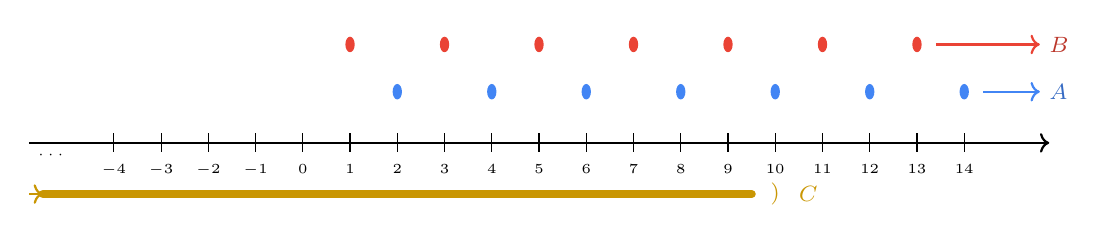
\begin{tikzpicture}[xscale=0.6, font=\small]
  % axis
  \draw[->, thick] (-5.8,0) -- (15.8,0);
  \foreach \x in {-4,-3,...,14} {
    \draw (\x, 0.12) -- (\x, -0.12);
    \node[below, font=\tiny] at (\x, -0.15) {$\x$};
  }
  \node[font=\tiny] at (-5.3, -0.15) {$\cdots$};

  % A: positive evens (blue dots)
  \foreach \x in {2,4,6,8,10,12,14}
    \fill[setA] (\x, 0.65) circle (2.8pt);
  \draw[->, setA, thick] (14.4, 0.65) -- (15.6, 0.65);
  \node[right, setA!80!black, font=\footnotesize] at (15.6, 0.65) {$A$};

  % B: positive odds (red dots)
  \foreach \x in {1,3,5,7,9,11,13}
    \fill[setB] (\x, 1.25) circle (2.8pt);
  \draw[->, setB, thick] (13.4, 1.25) -- (15.6, 1.25);
  \node[right, setB!80!black, font=\footnotesize] at (15.6, 1.25) {$B$};

  % C: x < 10 (yellow bar)
  \draw[setC!80!black, line width=3pt, line cap=round]
    (-5.5, -0.65) -- (9.5, -0.65);
  \draw[<-, setC!80!black, thick] (-5.5, -0.65) -- (-5.8, -0.65);
  \node[setC!80!black, font=\footnotesize] at (10.0, -0.65) {$)$};
  \node[right, setC!80!black, font=\footnotesize] at (10.3, -0.65) {$C$};
\end{tikzpicture}
\end{center}

\textbf{Նախ թարգմանեք յուրաքանչյուր գործողություն բառերով.}
\begin{itemize}[nosep]
  \item $\comp{A}$: ամբողջ թվեր, որոնք դրական զույգ \textbf{չեն}։
  \item $A \symdiff B$: ամբողջ թվեր, որոնք $A, B$-ից \textbf{ճիշտ մեկում} են։
  \item $\comp{C}$: ամբողջ թվեր, որոնք $10$-ից փոքր \textbf{չեն}։
  \item $A \setminus C$: դրական զույգ թվեր, որոնք $C$-ում \textbf{չեն} (այսինքն՝ $\ge 10$)։
  \item $C \setminus (A \symdiff B)$: ամբողջ թվեր $< 10$, որոնք դրական \textbf{չեն}։
\end{itemize}

\medskip
\textbf{(a)\; $\comp{A}$:}\;
Ամեն ինչ $\Z$-ում, որը դրական զույգ ամբողջ թիվ \emph{չէ}։
\[
  \boxed{\comp{A} = \{\ldots, -2, -1, 0\} \;\cup\; \{1, 3, 5, 7, \ldots\}
         = \bigl\{x \in \Z \mid x \le 0 \text{ կամ } x \text{-ը կենտ է}\bigr\}}
\]

\textbf{(b)\; $A \symdiff B$:}\;
Քանի որ $A \cap B = \varnothing$ (ոչ մի ամբողջ թիվ միաժամանակ և՛ դրական զույգ չէ, և՛ դրական կենտ)․
\[
  A \symdiff B = A \cup B = \{1, 2, 3, 4, \ldots\}
\]
Քանի որ յուրաքանչյուր դրական ամբողջ թիվ կա՛մ զույգ է, կա՛մ կենտ (և երբեք միաժամանակ երկուսը լինել չի կարող), ստանում ենք $A \cup B = \Z^+$ և $A \cap B = \varnothing$։
\[
  \boxed{A \symdiff B = \Z^+}
\]

\textbf{(c)\; $\comp{C}$:}\;
Բոլոր ամբողջ թվերը $\ge 10$։
$\quad\boxed{\comp{C} = \{10, 11, 12, \ldots\}}$

\textbf{(d)\; $A \setminus C$:}\;
Դրական զույգ թվեր, որոնք $\ge 10$ են։
$\quad\boxed{A \setminus C = \{10, 12, 14, \ldots\} = \{2k \mid k \ge 5\}}$

\textbf{(e)\; $C \setminus (A \symdiff B)$:}\;
Սա բաղադրյալ գործողություն է։ կատարեք այն քայլ առ քայլ։

\begin{enumerate}[label=\textbf{Քայլ \arabic*։}, leftmargin=*, nosep, itemsep=4pt]
  \item \textbf{Հաշվեք ներքին փակագծերը.}\;
        $A \symdiff B$. Վերևի (b) մասից արդեն գիտենք
        $\boxed{A \symdiff B = \Z^+}$ (բոլոր դրական ամբողջ թվերը)։

  \item \textbf{Տեղադրեք արտաքին գործողության մեջ.}\;
        $C \setminus (A \symdiff B) = C \setminus \Z^+$.
        Սա նշանակում է՝ վերցնել $C$-ի բոլոր տարրերը (ամբողջ թվեր $< 10$) և
        հեռացնել յուրաքանչյուր դրական ամբողջ թիվ։

  \item \textbf{Հաշվեք արդյունքը.}\;
        $C$-ի տարրերը, որոնք դրական \emph{չեն},
        $\ldots, -2, -1, 0$ թվերն են։
\end{enumerate}
\[
  \boxed{C \setminus (A \symdiff B) = \{\ldots, -2, -1, 0\}
         = \{x \in \Z \mid x \le 0\}}
\]

% ══════════════════════════════════════════════════════════════════
\newpage
\section{Խնդիր 20 — $\subseteq$-ի համարժեք բնութագրեր}
% ══════════════════════════════════════════════════════════════════

\begin{theorybox}[Ցիկլային հետևության ապացուցման ռազմավարություն]
Ցույց տալու համար, որ երեք պայմաններ՝ $(a)$, $(b)$, $(c)$, համարժեք են, բավական է ապացուցել
\textbf{հետևությունների ցիկլ}։
\[
  (a) \;\Longrightarrow\; (b) \;\Longrightarrow\; (c) \;\Longrightarrow\; (a):
\]
Սա ավելի արդյունավետ է, քան բոլոր վեց զույգային հետևությունները ուղղակիորեն ապացուցելը։

\begin{center}
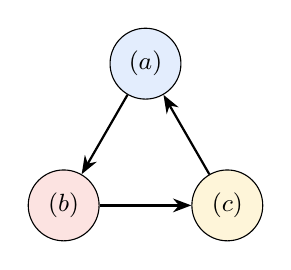
\begin{tikzpicture}[>=Stealth, font=\small]
  \node[draw, circle, minimum size=0.9cm, fill=setA!15] (a) at (90:1.2) {$(a)$};
  \node[draw, circle, minimum size=0.9cm, fill=setB!15] (b) at (210:1.2) {$(b)$};
  \node[draw, circle, minimum size=0.9cm, fill=setC!15] (c) at (330:1.2) {$(c)$};
  \draw[->, thick] (a) -- (b);
  \draw[->, thick] (b) -- (c);
  \draw[->, thick] (c) -- (a);
\end{tikzpicture}
\end{center}
\end{theorybox}

\begin{problembox}
Ապացուցեք, որ $U$ ունիվերսալ բազմության ցանկացած $A, B$ ենթաբազմությունների համար
յուրաքանչյուր խմբի պայմանները համարժեք են․
\begin{enumerate}[nosep]
  \item $A \subseteq B \;\iff\; A \cup B = B \;\iff\; A \cap B = A$
  \item $A \cap B = \varnothing \;\iff\; A \subseteq \comp{B} \;\iff\; B \subseteq \comp{A}$
  \item $A \cup B = U \;\iff\; \comp{A} \subseteq B \;\iff\; \comp{B} \subseteq A$
\end{enumerate}
\end{problembox}

\begin{tcolorbox}[colback=theoryBg, colframe=theoryFrame!80!black, arc=2mm, left=5pt, right=5pt, top=5pt, bottom=5pt, title={\small Տեսողական ինտուիցիա. Ինչո՞ւ են այս պայմանները համարժեք}]
Նախքան ֆորմալ ապացույցին անցնելը, դիտարկեք այս Վենի դիագրամը, որը ցույց է տալիս $A \subseteq B$ (այսինքն՝ $A$-ն ամբողջությամբ գտնվում է $B$-ի ներսում)․

\begin{center}
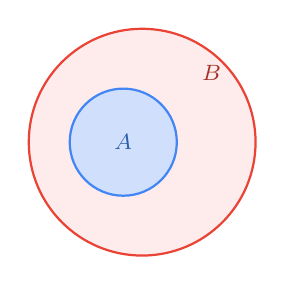
\begin{tikzpicture}[scale=0.8]
  \draw[thick, setB, fill=setB!10] (0,0) circle (1.8);
  \draw[thick, setA, fill=setA!25] (-0.3,0) circle (0.85);
  \node[font=\footnotesize\bfseries, setA!70!black] at (-0.3,0) {$A$};
  \node[font=\footnotesize\bfseries, setB!70!black] at (1.1,1.1) {$B$};
\end{tikzpicture}
\end{center}

\begin{itemize}[nosep]
  \item \textbf{Ինչո՞ւ $A \cup B = B$։} Քանի որ $A$-ն արդեն $B$-ի ներսում է, $A$-ն միավորմանը ավելացնելը ոչինչ չի փոխում։ $A \cup B$-ի ստվերագծված տիրույթը ուղղակի $B$-ն է։
  \item \textbf{Ինչո՞ւ $A \cap B = A$։} $A$-ի յուրաքանչյուր տարր նաև $B$-ում է (քանի որ $A$-ն $B$-ի ներսում է), ուստի $B$-ի հետ հատումը պահպանում է ամբողջ $A$-ն։ $A$-ից ոչինչ չի հեռացվում։
\end{itemize}

Այս պատկերը ստեղծում է տպավորություն, որ բոլոր երեք պայմանները նույն պնդումն են տարբեր բառերով։ Ստորև բերված ֆորմալ ցիկլային հետևության ապացույցը խստորեն հաստատում է դա։
\end{tcolorbox}

% ---- Part 1 ----
\subsection*{Մաս 1.\; $A \subseteq B \;\iff\; A \cup B = B \;\iff\; A \cap B = A$}

\begin{center}
\begin{tikzpicture}[scale=0.72]
  % A subset B
  \draw[thick, setB, fill=setB!10] (0,0) circle (1.6);
  \draw[thick, setA, fill=setA!20] (-0.3,0) circle (0.8);
  \node[font=\footnotesize\bfseries, setA!70!black] at (-0.3,0) {$A$};
  \node[font=\footnotesize\bfseries, setB!70!black] at (0.9,1.0) {$B$};
  \node[font=\footnotesize] at (0, -2.2) {$A \subseteq B$};

  \begin{scope}[xshift=4.5cm]
    \draw[thick, setB, fill=setB!25] (0,0) circle (1.6);
    \draw[thick, setA, dashed] (-0.3,0) circle (0.8);
    \node[font=\footnotesize] at (0, -2.2) {$A \cup B = B$};
    \node[font=\footnotesize, setB!70!black] at (0,0) {ամբողջ $B$-ն};
  \end{scope}

  \begin{scope}[xshift=9cm]
    \draw[thick, setB, dashed] (0,0) circle (1.6);
    \draw[thick, setA, fill=setA!25] (-0.3,0) circle (0.8);
    \node[font=\footnotesize] at (0, -2.2) {$A \cap B = A$};
    \node[font=\footnotesize, setA!70!black] at (-0.3,0) {$A$};
  \end{scope}

  % arrows between diagrams
  \draw[<->, thick, gray] (1.9, 0) -- (2.6, 0);
  \draw[<->, thick, gray] (6.4, 0) -- (7.1, 0);
\end{tikzpicture}
\end{center}

\smallskip
\textit{Հիմնական գաղափար. եթե $A$-ն արդեն $B$-ի ներսում է, $A$-ն միավորմանը ավելացնելը ոչինչ չի փոխում, իսկ $B$-ի հետ հատումը պահպանում է ամբողջ $A$-ն։}

\smallskip
\textbf{$(a) \Rightarrow (b)$։}\;
$A \subseteq B \;\Longrightarrow\; A \cup B = B$.

($\supseteq$)\; $B \subseteq A \cup B$ միշտ։

($\subseteq$)\; Դիցուք $x \in A \cup B$։
Ապա $x \in A$ կամ $x \in B$։
Եթե $x \in A$, ապա $A \subseteq B$-ից հետևում է $x \in B$։
Ցանկացած դեպքում $x \in B$։ \qed

\textbf{$(b) \Rightarrow (c)$։}\;
$A \cup B = B \;\Longrightarrow\; A \cap B = A$.

($\subseteq$)\; $A \cap B \subseteq A$ միշտ։

($\supseteq$)\; Դիցուք $x \in A$։
Ապա $x \in A \cup B = B$, ուստի $x \in B$։
Հետևաբար $x \in A \cap B$։ \qed

\textbf{$(c) \Rightarrow (a)$։}\;
$A \cap B = A \;\Longrightarrow\; A \subseteq B$.

Դիցուք $x \in A$։ Ապա $x \in A = A \cap B$, ուստի $x \in B$։ \qed

% ---- Part 2 ----
\subsection*{Մաս 2.\; $A \cap B = \varnothing \;\iff\; A \subseteq \comp{B} \;\iff\; B \subseteq \comp{A}$}

\begin{center}
\begin{tikzpicture}[scale=0.72]
  \draw[thick, gray] (-2.3,-1.7) rectangle (2.3,1.7);
  \node[gray, font=\scriptsize] at (2.0,1.45) {$U$};
  \draw[thick, setA, fill=setA!20] (-0.85,0) circle (0.9);
  \draw[thick, setB, fill=setB!20] (0.85,0) circle (0.9);
  \node[font=\footnotesize\bfseries, setA!70!black] at (-0.85,0) {$A$};
  \node[font=\footnotesize\bfseries, setB!70!black] at (0.85,0) {$B$};
  \node[font=\footnotesize] at (0,-2.3) {Չհատվող. $A \cap B = \varnothing$};
  \node[font=\scriptsize, gray] at (0, 0) {$\varnothing$};
\end{tikzpicture}
\end{center}

\smallskip
\textit{Հիմնական գաղափար. չհատվող լինելը նշանակում է՝ $A$-ի յուրաքանչյուր տարր գտնվում է $B$-ից դուրս, այսինքն՝ $\comp{B}$-ում։}

\smallskip
\textbf{$(a) \Rightarrow (b)$։}\;
$A \cap B = \varnothing \;\Longrightarrow\; A \subseteq \comp{B}$.

Դիցուք $x \in A$։ Եթե $x \in B$, ապա $x \in A \cap B = \varnothing$, ինչը հակասություն է։
Ուստի $x \notin B$, այսինքն՝ $x \in \comp{B}$։ \qed

\textbf{$(b) \Rightarrow (c)$։}\;
$A \subseteq \comp{B} \;\Longrightarrow\; B \subseteq \comp{A}$.

Դիցուք $x \in B$։ Եթե $x \in A$, ապա $x \in \comp{B}$ (քանի որ $A \subseteq \comp{B}$),
ուստի $x \notin B$, ինչը հակասություն է։ Հետևաբար $x \notin A$, այսինքն՝ $x \in \comp{A}$։ \qed

\textbf{$(c) \Rightarrow (a)$։}\;
$B \subseteq \comp{A} \;\Longrightarrow\; A \cap B = \varnothing$.

Ենթադրենք $x \in A \cap B$։ Ապա $x \in B \subseteq \comp{A}$,
ուստի $x \notin A$, ինչը հակասում է $x \in A \cap B$-ին։ \qed

% ---- Part 3 ----
\subsection*{Մաս 3.\; $A \cup B = U \;\iff\; \comp{A} \subseteq B \;\iff\; \comp{B} \subseteq A$}

\begin{center}
\begin{tikzpicture}[scale=0.72]
  % Shading: entire U is covered
  \draw[thick, gray, fill=gray!8] (-2.3,-1.7) rectangle (2.3,1.7);
  \node[gray, font=\scriptsize] at (2.0,1.45) {$U$};
  \fill[setA!20] (-0.5,0) circle (1.1);
  \fill[setB!20] (0.5,0) circle (1.1);
  % overlap
  \begin{scope}
    \clip (-0.5,0) circle (1.1);
    \fill[purple!15] (0.5,0) circle (1.1);
  \end{scope}
  \draw[thick, setA] (-0.5,0) circle (1.1);
  \draw[thick, setB] (0.5,0) circle (1.1);
  \node[font=\footnotesize\bfseries, setA!70!black] at (-1.1,0) {$A$};
  \node[font=\footnotesize\bfseries, setB!70!black] at (1.1,0) {$B$};
  \node[font=\footnotesize] at (0,-2.3) {Ծածկում. $A \cup B = U$};
\end{tikzpicture}
\end{center}

\smallskip
\textit{Հիմնական գաղափար. եթե $A$-ն և $B$-ն միասին ծածկում են $U$-ն, ապա $A$-ից դուրս ցանկացած բան պետք է լինի $B$-ում։}

\smallskip
\textbf{$(a) \Rightarrow (b)$։}\;
$A \cup B = U \;\Longrightarrow\; \comp{A} \subseteq B$.

Դիցուք $x \in \comp{A}$, այսինքն՝ $x \notin A$։
Քանի որ $x \in U = A \cup B$ և $x \notin A$, ապա պետք է, որ $x \in B$։ \qed

\textbf{$(b) \Rightarrow (c)$։}\;
$\comp{A} \subseteq B \;\Longrightarrow\; \comp{B} \subseteq A$.

Դիցուք $x \in \comp{B}$, այսինքն՝ $x \notin B$։
Եթե $x \notin A$, ապա $x \in \comp{A} \subseteq B$, ինչը տալիս է $x \in B$, որը հակասություն է։
Ուստի $x \in A$։ \qed

\textbf{$(c) \Rightarrow (a)$։}\;
$\comp{B} \subseteq A \;\Longrightarrow\; A \cup B = U$.

Դիցուք $x \in U$։ Կա՛մ $x \in B$ (այդ դեպքում $x \in A \cup B$),
կա՛մ $x \notin B$ (այդ դեպքում $x \in \comp{B} \subseteq A$, ուստի $x \in A \cup B$)։
Քանի որ նաև $A \cup B \subseteq U$, ստանում ենք $A \cup B = U$։ \qed

% ══════════════════════════════════════════════════════════════════
\newpage
\section{Խնդիր 54.3 — $(A \cup B) \setminus C = (A \setminus C) \cup (B \setminus C)$}
% ══════════════════════════════════════════════════════════════════

\begin{theorybox}[Տարբերության բաշխականությունը միավորման նկատմամբ]
Մտավոր մոդել. «$X \setminus C$» նշանակում է
«սկսիր $X$-ից, \textbf{հեռացրու} այն ամենը, ինչ $C$-ում է»։

Միավորումից $C$ բազմությունը հեռացնելը համարժեք է յուրաքանչյուր բազմությունից այն առանձին հեռացնելուն և ստացված մնացորդները միավորելուն։

\begin{center}
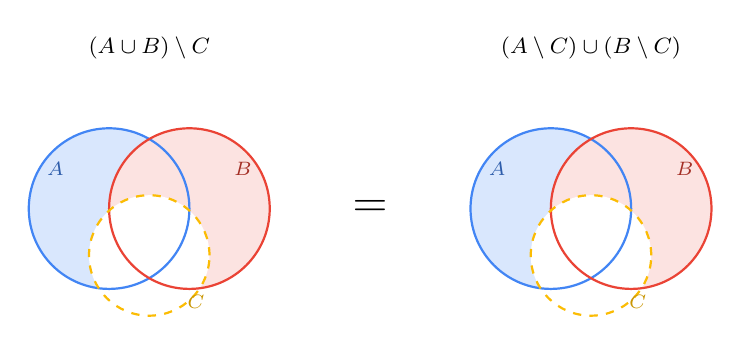
\begin{tikzpicture}[scale=0.85]
  % --- LHS ---
  \begin{scope}[xshift=0cm]
    \node[font=\footnotesize\bfseries] at (0, 2.4) {$(A \cup B) \setminus C$};
    % shade A\C
    \begin{scope}
      \clip (-0.6,0) circle (1.2);
      \fill[setA!20] (-3,-3) rectangle (3,3);
    \end{scope}
    % shade B\C
    \begin{scope}
      \clip (0.6,0) circle (1.2);
      \fill[setB!15] (-3,-3) rectangle (3,3);
    \end{scope}
    % cut out C
    \fill[white] (0, -0.7) circle (0.9);

    \draw[thick, setA] (-0.6, 0) circle (1.2);
    \draw[thick, setB] (0.6, 0) circle (1.2);
    \draw[thick, setC, dashed] (0, -0.7) circle (0.9);
    \node[font=\scriptsize, setA!70!black] at (-1.4, 0.6) {$A$};
    \node[font=\scriptsize, setB!70!black] at (1.4, 0.6) {$B$};
    \node[font=\scriptsize, setC!80!black] at (0.7, -1.4) {$C$};
  \end{scope}

  \node[font=\LARGE] at (3.3, 0) {$=$};

  % --- RHS ---
  \begin{scope}[xshift=6.6cm]
    \node[font=\footnotesize\bfseries] at (0, 2.4) {$(A \setminus C) \cup (B \setminus C)$};
    % shade A\C
    \begin{scope}
      \clip (-0.6,0) circle (1.2);
      \fill[setA!20] (-3,-3) rectangle (3,3);
    \end{scope}
    % shade B\C
    \begin{scope}
      \clip (0.6,0) circle (1.2);
      \fill[setB!15] (-3,-3) rectangle (3,3);
    \end{scope}
    % cut out C
    \fill[white] (0, -0.7) circle (0.9);

    \draw[thick, setA] (-0.6, 0) circle (1.2);
    \draw[thick, setB] (0.6, 0) circle (1.2);
    \draw[thick, setC, dashed] (0, -0.7) circle (0.9);
    \node[font=\scriptsize, setA!70!black] at (-1.4, 0.6) {$A$};
    \node[font=\scriptsize, setB!70!black] at (1.4, 0.6) {$B$};
    \node[font=\scriptsize, setC!80!black] at (0.7, -1.4) {$C$};
  \end{scope}
\end{tikzpicture}
\end{center}
Երկու դիագրամները ստվերագծում են ճիշտ նույն տիրույթը՝ $A$-ի և $B$-ի այն մասերը,
որոնք $C$-ից դուրս են։
\end{theorybox}

\begin{problembox}
Ապացուցեք․\quad $(A \cup B) \setminus C = (A \setminus C) \cup (B \setminus C)$։
\end{problembox}

\subsection*{Լուծում}

Դիցուք $x$-ը կամայական է․
\begin{align*}
  x \in (A \cup B) \setminus C
  &\iff x \in (A \cup B) \;\land\; x \notin C \\
  &\iff (x \in A \;\lor\; x \in B) \;\land\; x \notin C \\
  &\iff (x \in A \land x \notin C)
        \;\lor\; (x \in B \land x \notin C)
        && \text{($\land$-ը բաշխվում է $\lor$-ի նկատմամբ)} \\
  &\iff x \in (A \setminus C) \;\lor\; x \in (B \setminus C) \\
  &\iff x \in (A \setminus C) \cup (B \setminus C):
\end{align*}
Յուրաքանչյուր քայլ $\iff$ է, ուստի բազմությունները հավասար են։ \qed

\smallskip
\textbf{Բազմությունների լեզվով ընթերցում.}\; «$C$-ից դուրս» լինելը «$A$-ում կամ $B$-ում»-ի վրա բաշխելը տրամաբանական $p \land (q \lor r) \iff (p \land q) \lor (p \land r)$ օրենքի բազմությունների տարբերակն է։

\medskip
\begin{tcolorbox}[colback=theoryBg, colframe=theoryFrame!80!black, arc=2mm, left=5pt, right=5pt, top=5pt, bottom=5pt, title={\small Տիրույթների համարակալման մեթոդ — Էմպիրիկ ստուգում}]
\textbf{Տեխնիկա.}\; Երեք բազմությամբ Վենի դիագրամում կան $2^3 = 8$ տիրույթներ։
Համարակալեք դրանք ըստ այն բանի, թե որ բազմություններին են պատկանում․

\begin{center}
\renewcommand{\arraystretch}{1.2}
\begin{tabular}{cl}
\toprule
\textbf{Տիրույթ} & \textbf{Պատկանելիություն} \\
\midrule
1 & միայն $A$ \\
2 & միայն $B$ \\
3 & միայն $C$ \\
4 & միայն $A \cap B$ ($C$-ում չէ) \\
5 & միայն $A \cap C$ ($B$-ում չէ) \\
6 & միայն $B \cap C$ ($A$-ում չէ) \\
7 & $A \cap B \cap C$ \\
8 & Ոչ մեկը ($\comp{A} \cap \comp{B} \cap \comp{C}$) \\
\bottomrule
\end{tabular}
\end{center}

Այժմ արտահայտենք հավասարության յուրաքանչյուր կողմն ըստ իր տիրույթների համարների։
\begin{itemize}[nosep]
  \item $A \cup B = \{1, 2, 4, 5, 6, 7\}$
  \item $(A \cup B) \setminus C$: հեռացնել $C$-ի տիրույթները ($\{3,5,6,7\}$)
        $\;\Longrightarrow\; \boxed{\{1, 2, 4\}}$
  \item $A \setminus C = \{1, 4\}$, \quad $B \setminus C = \{2, 4\}$
  \item $(A \setminus C) \cup (B \setminus C) = \{1, 4\} \cup \{2, 4\} = \boxed{\{1, 2, 4\}}$
\end{itemize}

Երկու կողմերն էլ տալիս են ճիշտ նույն տիրույթները $\{1, 2, 4\}$, ինչը էմպիրիկորեն հաստատում է նույնությունը։

\medskip
\textit{Այս մեթոդը չի փոխարինում ապացույցին, բայց հիանալի միջոց է վստահություն ձեռք բերելու կամ սխալները հայտնաբերելու համար նախքան ապացույցը գրելը։}
\end{tcolorbox}

\end{document}